\subsection{Проектирование архитектуры программного средства}

При проектировании программного средства изначально была выбранна микросервисная архитектура, которая позволяет разбить приложение
на независимые модули, которые могут быть разработаны и протестированы отдельно друг от друга. 
Это позволяет упростить процесс разработки и тестирования, а также улучшить масштабируемость приложения.

\subsubsection{Схема взаимодействия микросервисов}

В процессе проектирования было определено, что необходимо реализовать следующие микросервисы:
\begin{itemize}
    \item микросервис для работы с пользователями;
    \item микросервис для работы с задачами;
    \item микросервис для работы с логированием;
\end{itemize}

Под каждый микросервис будет разрабатываться в отдельной ветке mono-репозитория с настроеным CI/CD для проверки сборки микросервиса
и отправки его в Docker Hub хранилище для последующего использования.

Схема взаимодействия микросервисов представлена на рисунке \ref{fig:main}.

\begin{figure}[ht]
    \centering
    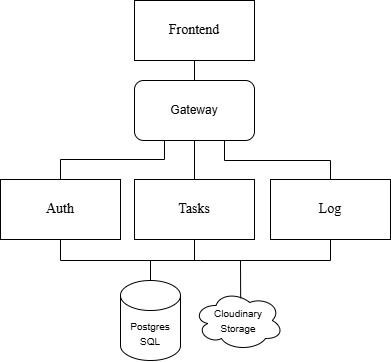
\includegraphics[width=0.60\linewidth]{\commonSecPathPrefix/sec_2/content/main_arch.png}
    \caption{Общая схема взаимодейсвия микросервисов}
    \label{fig:main}
\end{figure}

Для упрощения работы с API на строноне клиент было решено настроить и использовать API Gateway, который будет служить proxy сервером для
всех запросов к микросервисам.

\subsubsection{Брокер сообщений}

Для распределения нагрузки между микросервисами и обеспечения их взаимодействия без нагрузки на Gateway был внедрён брокер сообщений
Kafka \cite{kafkaDocs}. Для правильной работы с брокером сообщений необходимо также использовать Zookeeper, который будет хранить
конфигурацию брокера и обеспечивать его работу.

Схема работы брокера сообщений представлена на рисунке \ref{fig:kafka}.

\begin{figure}[ht]
    \centering
    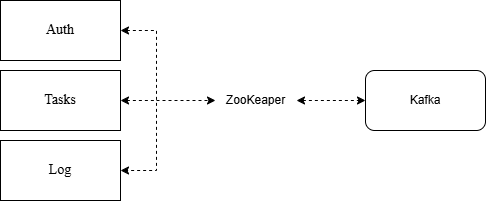
\includegraphics[width=0.60\linewidth]{\commonSecPathPrefix/sec_2/content/kafka.png}
    \caption{Схема взаимодейсвия брокера сообщений}
    \label{fig:kafka}
\end{figure}

Zookeeper служит средством распределения нагрузки между брокерами путём выделения лидера который будет обрабатывать все запросы,
что является необходимым условием для работы брокера сообщений.

\subsubsection{Логирование}

Для удобного и быстрого получения информации о состоянии системы в неё внедряются системы логирования.
В данном случае будет использоваться ELK набор, состоящий из следующих компонентов:
\begin{itemize}
    \item Elasticsearch - система хранения и поиска данных;
    \item Logstash - система сбора и обработки логов;
    \item Kibana - система визуализации данных;
\end{itemize}

Схема работы системы логирования представлена на рисунке \ref{fig:kibana}.

\begin{figure}[ht]
    \centering
    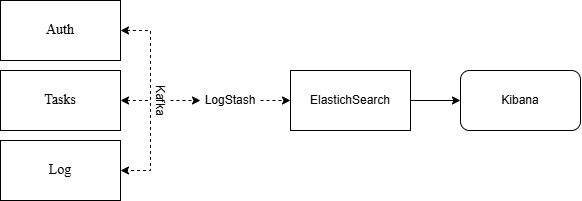
\includegraphics[width=0.60\linewidth]{\commonSecPathPrefix/sec_2/content/kibana.png}
    \caption{Схема работы логирования}
    \label{fig:kibana}
\end{figure}

Logstash перехватывает сообщения из Kafka с определённым заголовком и отправляет их в Elasticsearch, который хранит их в своей базе данных.
Для более удобного поиска, фильтрации и визуализации данных можно использовать Kibana \cite{kibanaDocs}. Функционал Kibana позволяет визуализировать данные
в виде графиков, таблиц и прочих элементов, что позволяет быстро и удобно получить информацию о состоянии системы.